\documentclass{article}

\usepackage{amsmath}
\usepackage{graphicx}

\begin{document}
\title{MCMD w2 -- Stellar population with clusters}
\author{Alex Arash Sand Kalaee\\ \texttt{kalaee@teorfys.lu.se}}
\maketitle
\section{First exercise}
We are provided as series of power law probability distributions
of the stellar masses $m$ in a cluster.
Using Monte Carlo importance sampling with the function $g(m) = m^{-2.2}$
we construct a random number generator for the masses according to the
specified distribution.

A star will explode as a supernova if its mass is above 8 sun masses.
We wish determine the probability for a cluster to contain at least one
supernova explosion according to the size of the cluster.
We generate 10000 different clusters for each size and sample the
statistics.
For the cluster sizes $N_*=$ 100, 300 and 1000 the probabilities are
0.30, 0.67 and 0.98 respectively.

The probabilities for clusters in the range 50 to 5000 stars are provided
in Fig~\ref{supernova}.

\begin{figure}
\centering
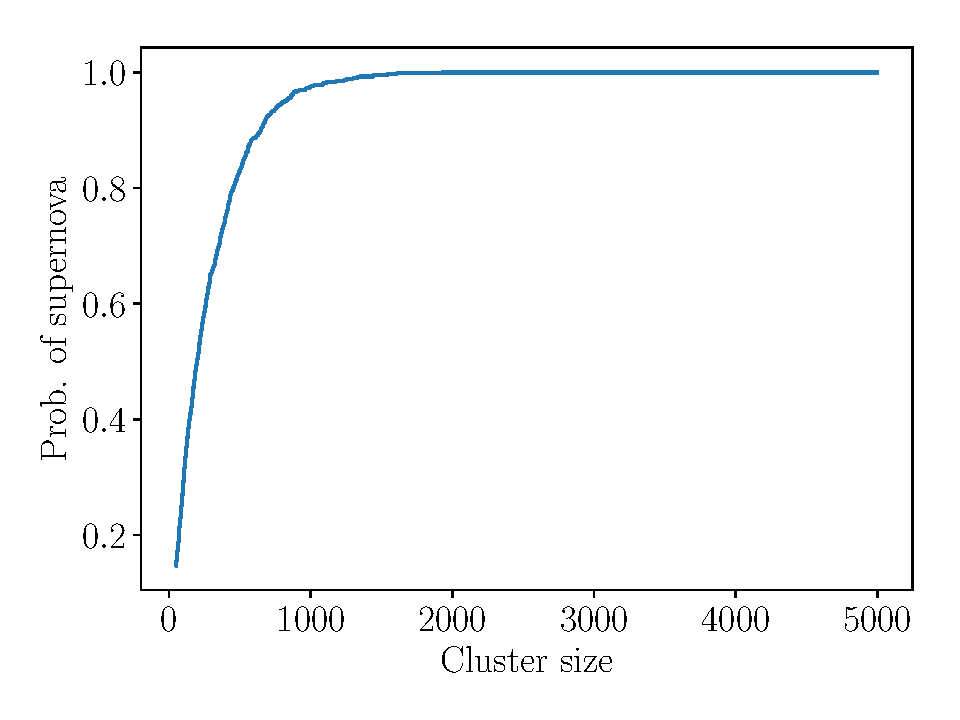
\includegraphics[width=0.8\textwidth]{supernova.pdf}
\caption{Probability for the cluster to contain a supernova. Estimated from
10000 different clusters per size.}
\label{supernova}
\end{figure}

I a cluster of 5000 stars we sample the number of supernova exploding stars
and find a mean and median of 18 stars, the lower quartile is 15 and the
upper quartile is 21 stars.

We are told our sun is believed to have formed in cluster with containing
material from a star with mass above 25 solar masses.
Sampling the presence of stars with masses above 25 solar masses from clusters
of different sizes, again with 10000 iterations for each size, we find that
the probability of having at least a single star above that threshold is
above 0.1 for $N_*\geq212$, above 0.25 for clusters
with $N_*\geq568$ and above 0.5 for clusters with $N_*\geq1390$.
Without further knowledge of the probability distribution of different cluster
sizes the na\"ive analysis above yields the expectation that the cluster
which hosted the sun probably contained 1390 or more stars.

\section{Follow up}
We now consider clusters each with a million different stars, and generate
10000 different iterations of this cluster size. These are time evolved over
15 Gyr in steps of 1 Gyr.

The mean, upper and lower quantile for the populations of main sequence stars,
black holes, neutron stars and white dwarfs are provided in
Fig~\ref{ms}-\ref{wd} respectively. Note that due to the large cluster
size, the prob. distribution is sharply peaked, as evidenced
by the narrow quartile ranges. Only the distribution of black holes has
a noticeable interquartile range which makes sense given that black hole
masses are furthest away in the tail of the distribution.

After 12 Gyr the mean number of objects are 857964 main sequence stars,
350 black holes, 3280 neutron stars and 138405 white dwarfs.

\begin{figure}
\centering
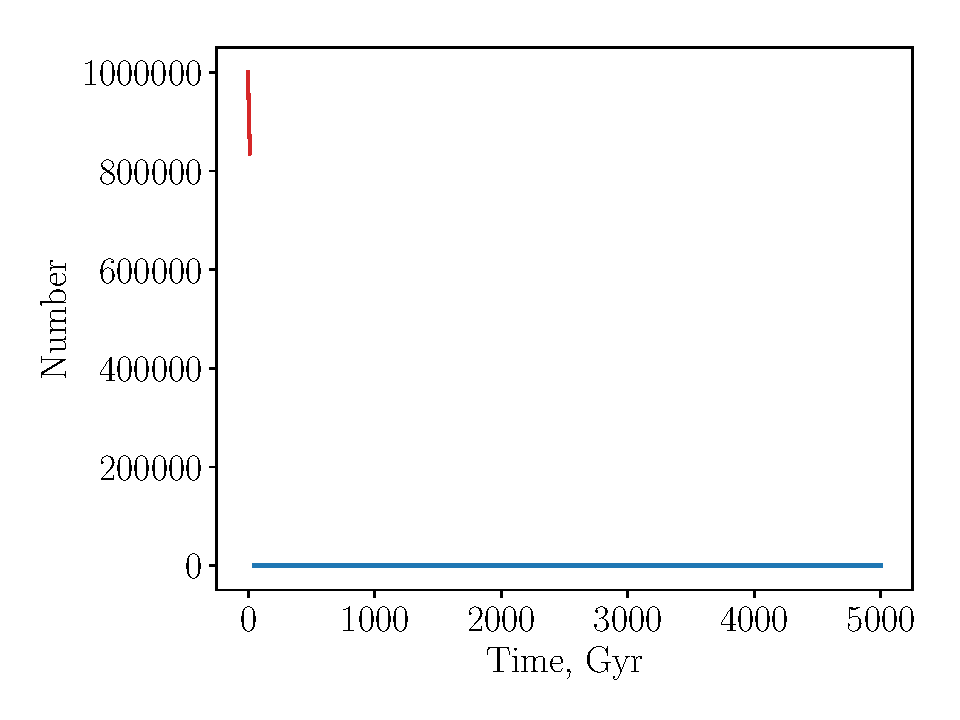
\includegraphics[width=0.8\textwidth]{ms.pdf}
\caption{Population of main sequence stars.}
\label{ms}
\end{figure}

\begin{figure}
\centering
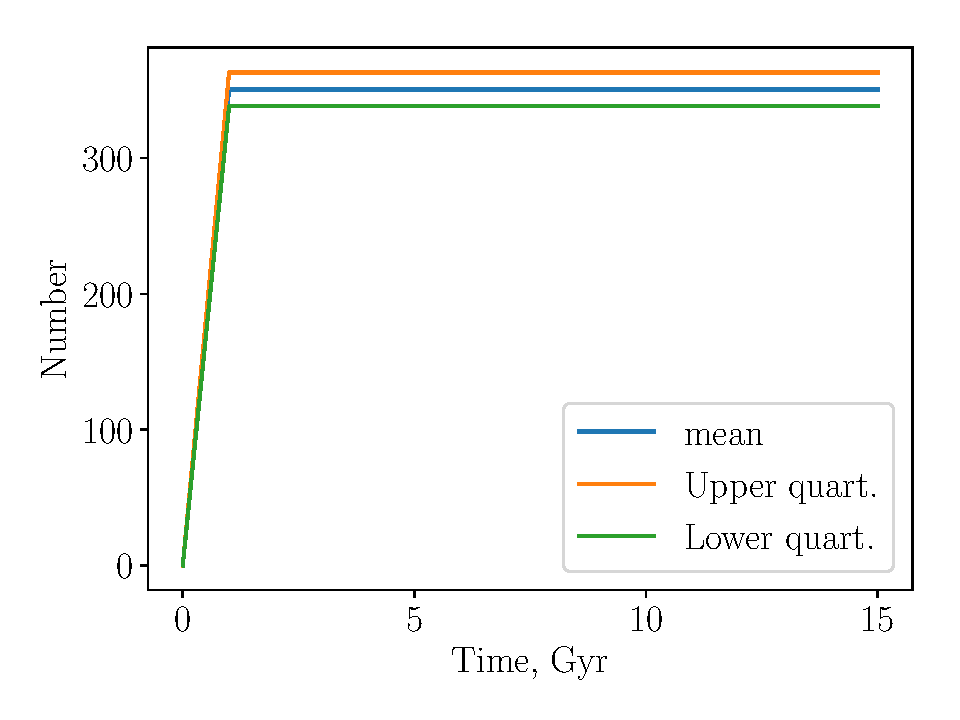
\includegraphics[width=0.8\textwidth]{bh.pdf}
\caption{Population of black holes.}
\label{bh}
\end{figure}

\begin{figure}
\centering
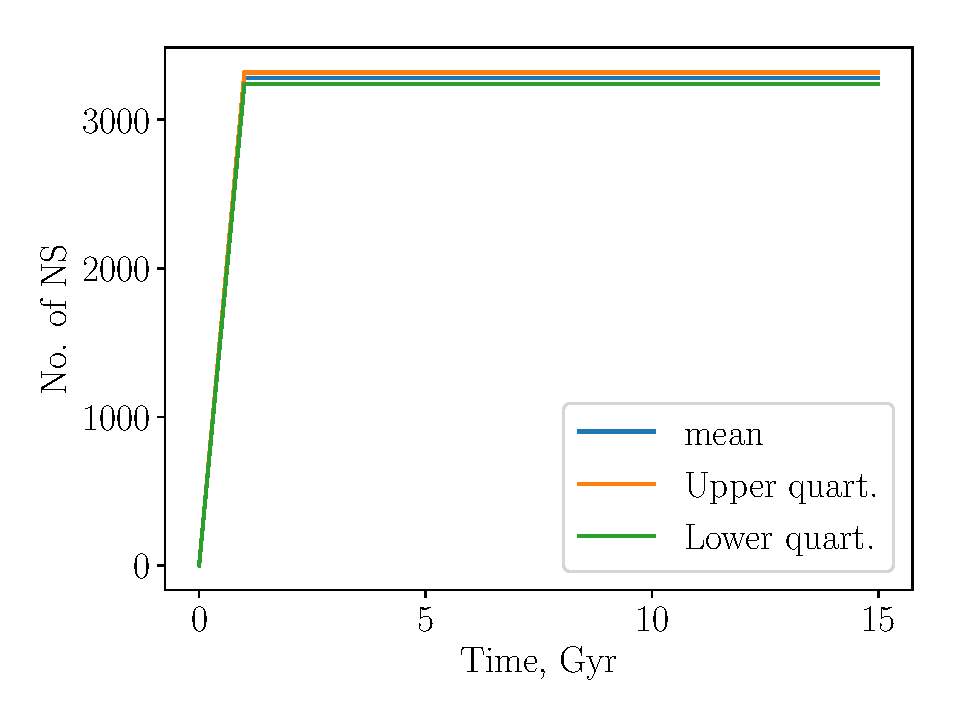
\includegraphics[width=0.8\textwidth]{ns.pdf}
\caption{Population of neutron stars.}
\label{ns}
\end{figure}

\begin{figure}
\centering
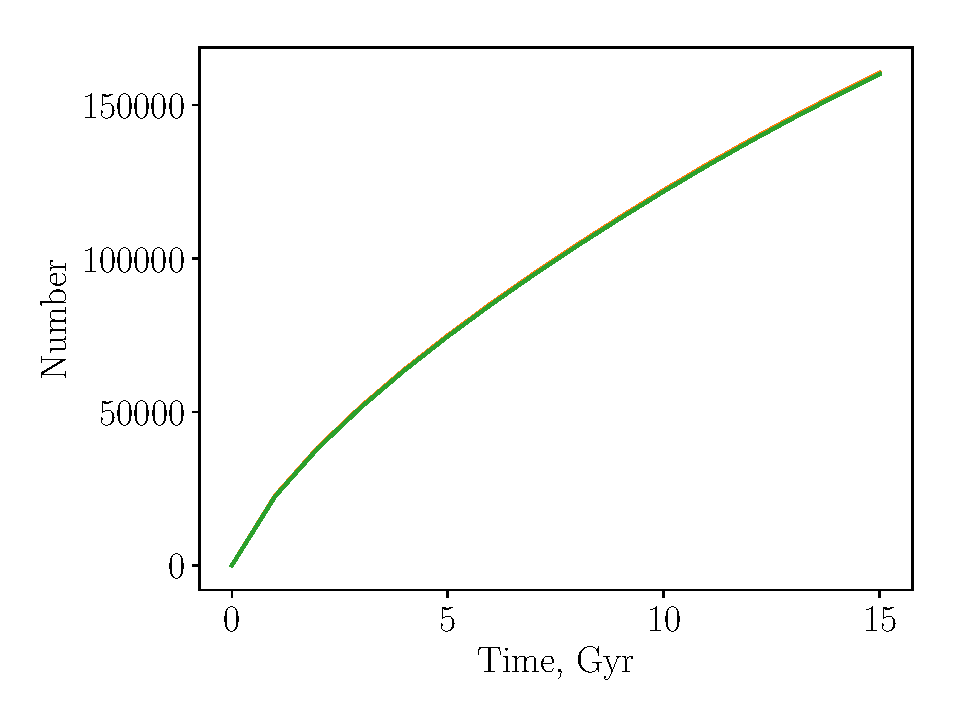
\includegraphics[width=0.8\textwidth]{wd.pdf}
\caption{Population of white dwarfs.}
\label{wd}
\end{figure}

We also find the total mass and luminosity ratio for the cluster as a function
of time, see Fig.~\ref{sm}-\ref{lm}.

\begin{figure}
\centering
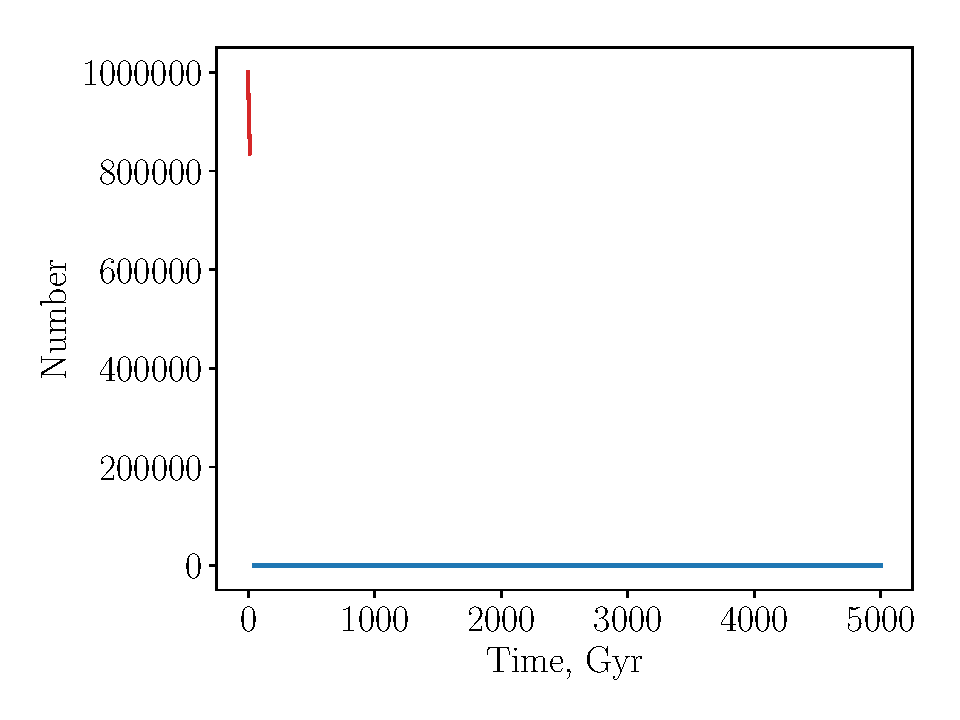
\includegraphics[width=0.8\textwidth]{ms.pdf}
\caption{Cluster mass.}
\label{sm}
\end{figure}

\begin{figure}
\centering
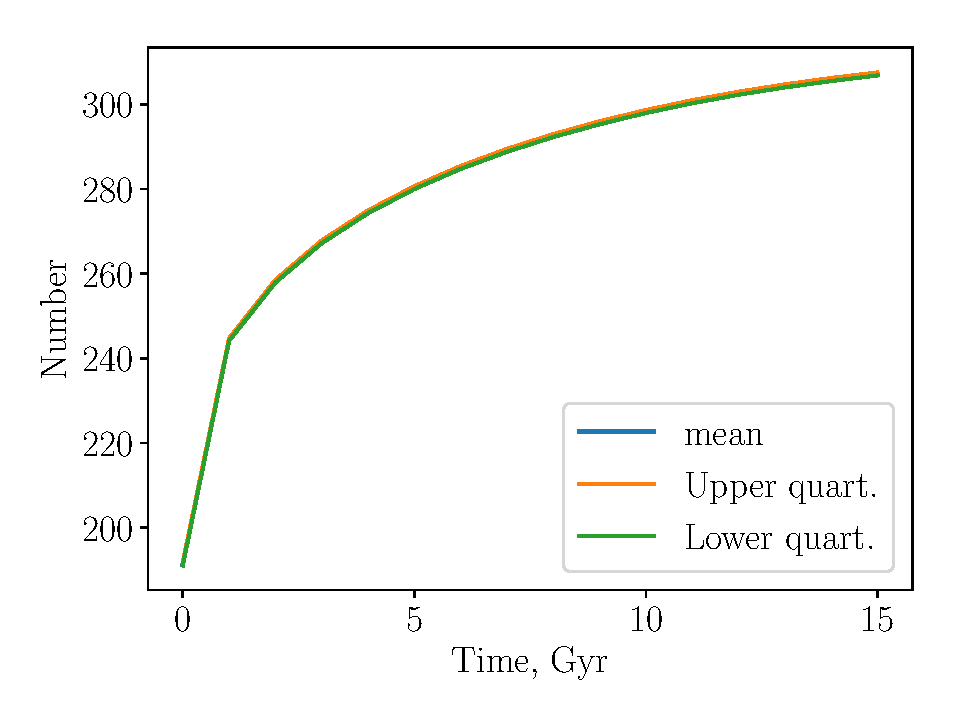
\includegraphics[width=0.8\textwidth]{lm.pdf}
\caption{Luminosity/mass ratio.}
\label{lm}
\end{figure}

\end{document}
